\documentclass[notheorems, hyperref]{beamer}

%% KEY LINES IN THIS TEX FILE %% (enter line number+gg to go)

%
% LOCAL FONT DEFINITIONS -- need to come first
%
%\usepackage{mathpazo}
%\usepackage{libertine}
%\usepackage[libertine]{newtxmath}
%\usefonttheme[onlymath]{serif}

%
% STANDARD PREAMBLE
%
%
% PACKAGES
%

\usepackage[T1]{fontenc}
% This uses 8-bit font encoding (with 256 glyphs) instead of the default 7-bit font encoding (with 128 glyphs). For example, with this option ö is a single glyph in the font, whereas on the 7-bit font encoding the font ö is made by adding an accent to the existing glyph o. A bad consequence of not using this package is that you cannot properly copy-paste such words form the output pdf file. Also, for some reason, funny stuff happens with |, < and > in text.

% Some people suggest to load fontenc before inputenc, most agree that it does not matter.

\usepackage[utf8]{inputenc}
% When you type ä in an editor set up for utf8, the machine stores the character number 228. When TeX reads the file it finds the character number 228 and the macros of inputenc transform this into \"a. Finally fontenc does its thing and transforms this into the command print character 228 (otherwise the two things would be printed separatedly as explained in fontenc).

\usepackage[UKenglish]{babel}
% To manage culturally determined typographical and similar rules, in this case for british english. Some people suggest to load babel after fontenc to avoid warnings, although most agree that it does not matter.

\usepackage{mathtools}
% Loads the amsmath package (\usepackage{amsmath}: miscellaneous improvements such as the commands \DeclareMathOperator and \text). It fixes some quirks it has and adds some useful settings, symbols and environments. It improves the aesthetics as well.

\usepackage{amssymb}
% Extended symbol collection, e.g. \Cap and \Cup. More importantly: the \mathbb command! It loads the amsfonts package (\usepackage{amsfonts}: fraktur letters, bold Greek letters...), so we do not need to include it in the preamble anymore.

\usepackage{mathrsfs}
% Font package (only supports upper case letters).

\usepackage{enumitem}
% To control the layout of enumerate, itemize and description. It supersedes the enumerate package.

\usepackage{tikz-cd}
% To draw commutative diagrams.
\usetikzlibrary{decorations.markings}
% For open and closed immersions.

\usepackage{graphicx}
% An extension of the graphics package, with optional arguments for the \includegraphics command.

\usepackage{todonotes}
% To write to do notes use the command \todo.

% \usepackage{xcolor}
% To write in colors.
% Already loaded by beamer class.

\usepackage{mathdots}
% To draw diagonal dots.

\usepackage{marginnote}
% To write on margins.

\usepackage{manfnt}
% To draw dangerous bent symbol.

\usepackage{float}
% Improved interface for floating objects such as figures and tables, introducing for example the H modifier to force the position of a float in the page or the boxed float. Should be loaded before hyperref.

% \usepackage[backref]{hyperref}
% To handle cross-referencing and produce hypertext links in the document. It should be loaded last (with few exceptions), because it redefines many LaTeX commands.
% The backref option inserts links on each bibliography entry to the pages in which the citation was used.
%% The hidelinks option removes colors and boxes around links, but the links remain clickable. On firefox the links are even highlighted when the mouse pointer passes over them.
% \renewcommand{\backref}[1]{$\uparrow$~#1}
% Adds an upwards arrow before referencing to the pages in which the citations appear.
% Already loaded by beamer class.

\usepackage[noabbrev]{cleveref}
% Enhances cross-referencing features, e.g. to reference to a theorem and automatically include the word theorem.
% No abbreviature option to write figure instead of fig. etc.

% Open and closed immersion arrows.
\makeatletter
\tikzcdset{
open/.code={\tikzcdset{hook, circled};},
closed/.code={\tikzcdset{hook, slashed};},
circled/.code={\tikzcdset{markwith={\draw (0,0) circle (.375ex);}};},
slashed/.code={\tikzcdset{markwith={\draw[-] (-.4ex,-.4ex) -- (.4ex,.4ex);}};},
markwith/.code={
\pgfutil@ifundefined{tikz@library@decorations.markings@loaded}%
{\pgfutil@packageerror{tikz-cd}{You need to say %
\string\usetikzlibrary{decorations.markings} to use arrow with markings}{}}{}%
\pgfkeysalso{/tikz/postaction={/tikz/decorate,
/tikz/decoration={
markings,
mark = at position 0.5 with
{#1}}}}},
}
\makeatother

% Custom colors
\definecolor{darkgreen}{RGB}{0,75,0}
\definecolor{darkblue}{RGB}{0,0,75}
\definecolor{darkred}{RGB}{75,0,0}
\definecolor{linkred}{rgb}{0.7,0.2,0.2}
\definecolor{linkblue}{rgb}{0,0.2,0.6}

% Limit table of contents to section titles
\setcounter{tocdepth}{1}

% Sloppy formatting -- often looks better
\sloppy

%
% FONT DEFINTIONS
%

% Script Font used for sheaves
\DeclareFontFamily{OMS}{rsfs}{\skewchar\font'60}
\DeclareFontShape{OMS}{rsfs}{m}{n}{<-5>rsfs5 <5-7>rsfs7 <7->rsfs10 }{}
\DeclareSymbolFont{rsfs}{OMS}{rsfs}{m}{n}
\DeclareSymbolFontAlphabet{\scr}{rsfs}
\DeclareSymbolFontAlphabet{\scr}{rsfs}

% Sheaves
\newcommand{\sA}{\scr{A}}
\newcommand{\sB}{\scr{B}}
\newcommand{\sC}{\scr{C}}
\newcommand{\sD}{\scr{D}}
\newcommand{\E}{\scr{E}} % Exception (Vector bundles)
\newcommand{\F}{\scr{F}} % Exception (Coherent sheaves)
\newcommand{\G}{\scr{G}} % Exception (Coherent sheaves)
\newcommand{\sH}{\scr{H}}
\renewcommand{\hom}{\scr{H}\negthinspace om} % Exception (Hom-sheaf)
\newcommand{\I}{\scr{I}} % Exception (Ideal sheaves)
\newcommand{\sJ}{\scr{J}}
\newcommand{\sK}{\scr{K}}
\renewcommand{\L}{\scr{L}} % Exception (Line bundles)
\newcommand{\M}{\scr{M}} % Exception (Line bundles)
\newcommand{\sN}{\scr{N}}
\renewcommand{\O}{\scr{O}} % Exception (Structure sheaf)
\newcommand{\sP}{\scr{P}}
\newcommand{\sQ}{\scr{Q}}
\newcommand{\sR}{\scr{R}}
\newcommand{\sS}{\scr{S}}
\newcommand{\sT}{\scr{T}}
\newcommand{\sU}{\scr{U}}
\newcommand{\sV}{\scr{V}}
\newcommand{\sW}{\scr{W}}
\newcommand{\w}{\omega} % Addition (Canonical sheaf)
\newcommand{\sX}{\scr{X}}
\newcommand{\sY}{\scr{Y}}
\newcommand{\sZ}{\scr{Z}}

% Mathcal fonts
\newcommand{\calA}{\mathcal{A}}
\newcommand{\calB}{\mathcal{B}}
\newcommand{\calC}{\mathcal{C}}
\newcommand{\calD}{\mathcal{D}}
\newcommand{\calE}{\mathcal{E}}
\newcommand{\calF}{\mathcal{F}}
\newcommand{\calG}{\mathcal{G}}
\newcommand{\calH}{\mathcal{H}}
\newcommand{\calI}{\mathcal{I}}
\newcommand{\calJ}{\mathcal{J}}
\newcommand{\calK}{\mathcal{K}}
\newcommand{\calL}{\mathcal{L}}
\newcommand{\calM}{\mathcal{M}}
\newcommand{\calN}{\mathcal{N}}
\newcommand{\calO}{\mathcal{O}}
\newcommand{\calP}{\mathcal{P}}
\newcommand{\calQ}{\mathcal{Q}}
\newcommand{\calR}{\mathcal{R}}
\newcommand{\calS}{\mathcal{S}}
\newcommand{\calT}{\mathcal{T}}
\newcommand{\U}{\mathcal{U}} % Exception (Open covers)
\newcommand{\calV}{\mathcal{V}}
\newcommand{\calW}{\mathcal{W}}
\newcommand{\X}{\mathcal{X}} % Exception (Families of varieties)
\newcommand{\Y}{\mathcal{Y}} % Exception (Families of varieties)
\newcommand{\calZ}{\mathcal{Z}}

% Blackboard Bold Symbols
\newcommand{\A}{\mathbb{A}} % Exception (Affine space)
\newcommand{\bbB}{\mathbb{B}}
\newcommand{\C}{\mathbb{C}} % Exception (Complex numbers)
\newcommand{\bbD}{\mathbb{D}}
\newcommand{\bbE}{\mathbb{E}}
\newcommand{\bbF}{\mathbb{F}}
\newcommand{\bbG}{\mathbb{G}}
\newcommand{\Gm}{\mathbb{G}_{\mathrm{m}}} % Addition (Punctured affine line)
\newcommand{\bbH}{\mathbb{H}}
\newcommand{\bbI}{\mathbb{I}}
\newcommand{\bbJ}{\mathbb{J}}
\newcommand{\bbK}{\mathbb{K}}
\renewcommand{\k}{\Bbbk} % Addition (Field)
\newcommand{\bbL}{\mathbb{L}}
\newcommand{\bbM}{\mathbb{M}}
\newcommand{\N}{\mathbb{N}} % Exception (Natural numbers)
\newcommand{\bbO}{\mathbb{O}}
\renewcommand{\P}{\mathbb{P}} % Exception (Projective space)
\newcommand{\Q}{\mathbb{Q}} % Exception (Rational numbers)
\newcommand{\R}{\mathbb{R}} % Exception (Real numbers)
\newcommand{\bbS}{\mathbb{S}}
\newcommand{\bbT}{\mathbb{T}}
\newcommand{\bbU}{\mathbb{U}}
\newcommand{\V}{\mathbb{V}} % Exception (Geometric vector bundle)
\newcommand{\bbW}{\mathbb{W}}
\newcommand{\bbX}{\mathbb{X}}
\newcommand{\bbY}{\mathbb{Y}}
\newcommand{\Z}{\mathbb{Z}} % Exception (Integers)

% Boldfont (categories)
\newcommand{\bfA}{\mathbf{A}}
\newcommand{\Ab}{\mathbf{Ab}}
\newcommand{\bfB}{\mathbf{B}}
\newcommand{\bfC}{\mathbf{C}}
\newcommand{\Cat}{\mathbf{Cat}} % Addition (Categories)
\newcommand{\Coh}{\mathbf{Coh}} % Addition (Coherent sheaves)
\newcommand{\D}{\mathbf{D}} % Exception (Derived category)
\newcommand{\Db}{\mathbf{D}^{\mathrm{b}}} % Addition (Bounded derived category)
\newcommand{\bfE}{\mathbf{E}}
\newcommand{\bfF}{\mathbf{F}}
\newcommand{\bfG}{\mathbf{G}}
\newcommand{\bfH}{\mathbf{H}}
\newcommand{\bfI}{\mathbf{I}}
\newcommand{\bfJ}{\mathbf{J}}
\newcommand{\K}{\mathbf{K}} % Exception (Homotopy category)
\newcommand{\bfL}{\mathbf{L}}
\newcommand{\bfM}{\mathbf{M}}
\newcommand{\Mod}{\mathbf{Mod}} % Addition (Modules)
\newcommand{\bfN}{\mathbf{N}}
\newcommand{\bfO}{\mathbf{O}}
\newcommand{\bfP}{\mathbf{P}}
\newcommand{\PSh}{\mathbf{PSh}} % Addition (Presheaves)
\newcommand{\bfQ}{\mathbf{Q}}
\newcommand{\QCoh}{\mathbf{QCoh}} % Addition (Quasi-coherent sheaves)
\newcommand{\bfR}{\mathbf{R}}
\newcommand{\bfS}{\mathbf{S}}
\newcommand{\Set}{\mathbf{Set}} % Addition (Sets)
\newcommand{\Sh}{\mathbf{Sh}} % Addition (Sheaves)
\newcommand{\bfT}{\mathbf{T}}
\renewcommand{\Top}{\mathbf{Top}} % Addition (Topological spaces)
\newcommand{\bfU}{\mathbf{U}}
\newcommand{\bfV}{\mathbf{V}}
\renewcommand{\Vec}{\mathbf{Vec}} % Addition (Vector bundles)
\newcommand{\bfW}{\mathbf{W}}
\newcommand{\bfX}{\mathbf{X}}
\newcommand{\bfY}{\mathbf{Y}}
\newcommand{\bfZ}{\mathbf{Z}}

% Mathfrak for ideals
\renewcommand{\a}{\mathfrak{a}}
\renewcommand{\b}{\mathfrak{b}}
\renewcommand{\c}{\mathfrak{c}}
\renewcommand{\d}{\mathfrak{d}}
\newcommand{\e}{\mathfrak{e}}
\newcommand{\m}{\mathfrak{m}}
\newcommand{\n}{\mathfrak{n}}

% Custom theorem styles (empty fields take default values)
\newtheoremstyle{darkgreentheorem}% name of the style
{}% measure of space to leave above the theorem. E.g.: 3pt
{}% measure of space to leave below the theorem. E.g.: 3pt
{\itshape}% name of font to use in the body of the theorem
{}% measure of space to indent
{\color{darkgreen}\bfseries}% name of head font
{}% punctuation between head and body
{ }% space after theorem head; " " = normal interword space
{}% Manually specify head
\newtheoremstyle{darkbluedefinition}
{}{}{}{}{\color{darkblue}\bfseries}{}{ }{}
\newtheoremstyle{darkredexample}
{}{}{}{}{\color{darkred}\bfseries}{}{ }{}



\allowdisplaybreaks

%
% ABOUT FONT DEFINTIONS IN THE PREAMBLE
%
% Mathscr for sheaves use \sA, where A can be any letter. Exceptions and additions:
% % \E (vector bundles)
% % \F (coherent sheaves)
% % \G (coherent sheaves)
% % \hom (sheaf hom)
% % \I (ideal sheaves)
% % \L (line bundles)
% % \M (line bundles)
% % \O (structure sheaf)
% % \w (canonical sheaf)
%
% Mathcal use \calA. Exceptions and additions:
% % \U (open cover)
% % \X (families of varieties)
% % \Y (families of varieties)
%
% Mathbb use \bbA. Exceptions and additions:
% % \A (affine space)
% % \C (complex numbers)
% % \Gm (puctured affine line)
% % \k (field)
% % \N (natural numbers)
% % \P (projective space)
% % \Q (rational numbers)
% % \R (real numbers)
% % \V (geometric vector bundle)
% % \Z (integers)
%
% Boldfont for categories use \bfA. Additions:
% % \Cat (categories)
% % \Coh (coherent sheaves)
% % \D (derived category)
% % \Db (bounded derived category)
% % \K (homotopy category)
% % \Mod (modules)
% % \PSh (presheaves)
% % \QCoh (quasi-coherent sheaves)
% % \Set (sets)
% % \Sh (sheaves)
% % \Top (topological spaces)
% % \Vec (vector bundles)
%
% Mathfrak for ideals
% % From \a to \e
% % \m and \n for maximal ideals

%
% THEOREM ENVIRONMENTS
%
% Theorems, propositions, etc (dark green)
\theoremstyle{darkgreentheorem}
\newtheorem{thm}{Theorem}
\newtheorem{reform}{Reformulation}
\newtheorem{lm}[thm]{Lemma}
\newtheorem{prop}[thm]{Proposition}
\newtheorem{cor}[thm]{Corollary}
\newtheorem{conj}[thm]{Conjecture}
% Definitions (dark blue)
\theoremstyle{darkbluedefinition}
\newtheorem{defn}[thm]{Definition}
% Examples (dark red)
\theoremstyle{darkredexample}
\newtheorem{exa}[thm]{Example}
% Remarks (black)
\theoremstyle{remark}
\newtheorem{rem}[thm]{Remark}
\newtheorem{nota}[thm]{Notation}
\newtheorem{fact}[thm]{Fact}
\newtheorem{q}[thm]{Question}
\newtheorem{pbl}[thm]{Problem}

%
% THEOREM CROSS-REFERENCING
%
\crefname{thm}{theorem}{theorems}
\Crefname{thm}{Theorem}{Theorems}
\crefname{lm}{lemma}{lemmas}
\Crefname{lm}{Lemma}{Lemmas}
\crefname{prop}{proposition}{propositions}
\Crefname{prop}{Proposition}{Propositions}
\crefname{cor}{corollary}{corollaries}
\Crefname{cor}{Corollary}{Corollaries}
\crefname{conj}{conjecture}{conjectures}
\Crefname{conj}{Conjecture}{Conjectures}
\crefname{defn}{definition}{definitions}
\Crefname{defn}{Definition}{Definitions}
\crefname{exa}{example}{examples}
\Crefname{exa}{Example}{Examples}
\crefname{rem}{remark}{remarks}
\Crefname{rem}{Remark}{Remarks}
\crefname{nota}{notation}{notations}
\Crefname{nota}{Notation}{Notations}
\crefname{fact}{fact}{facts}
\Crefname{fact}{Fact}{Facts}
\crefname{q}{question}{questions}
\Crefname{q}{Question}{Questions}
\crefname{pbl}{problem}{problems}
\Crefname{pbl}{Problem}{Problems}

%
% MATH OPERATORS
%
\DeclareMathOperator{\Hom}{Hom}
\DeclareMathOperator{\Pic}{Pic}

%
% OTHER COMMANDS
%
\newcommand{\ot}{\otimes}
\newcommand{\op}{\oplus}
\renewcommand{\L}{\mathcal{L}}
\renewcommand{\M}{\mathcal{M}}
\newcommand{\dual}{^{\vee}}

%
% TITLE PAGE INFORMATION
%
\title[Torelli's Theorem]{Torelli's Theorem}
\author{Remarks on Sections III.12--13 of Milne's \textit{Abelian Varieties}}
\institute{University of Freiburg}
\date{28th July 2020}
 
%
% LINKS AND PDF OPTIONS
%
\makeatletter
\hypersetup{
  %pdfauthor={\authors},
  pdftitle={\@title},
  %pdfsubject={\@subjclass},
  %pdfkeywords={\@keywords},
  %pdfstartview={Fit},
  %pdfpagelayout={TwoColumnRight},
  %pdfpagemode={UseOutlines},
  bookmarks,
  colorlinks,
  linkcolor=linkblue,
  citecolor=linkred,
  urlcolor=linkred}
\makeatother
\usecolortheme{rose}
 
\begin{document}
 
\frame{\titlepage}

\begin{frame}
    \frametitle{Assumptions, notation and recollections}
    \begin{enumerate}[label=\textbullet]
	\item $k$ is an algebraically closed field.
	    \pause
	\item $C$ is a smooth complete curve over $k$ of genus $g\geqslant 2$.
	    \pause
	\item $J$ is its Jacobian, which is an abelian variety representing
	    \[ T \mapsto \{ \L\in \Pic(C\times T) \mid \deg(\L_{t})=0 \text{ for all }t\in T \}/\Pic(T). \]
	    \vspace{-1em}
	    \pause
	\item In particular, we may and will identify $J(k)=\Pic^{0}(C)$.
	    \pause
	\item Fix $P\in C(k)$ once and for all.
	    Then we get a canonical map
	    \[ f\colon C\to J, \quad Q\mapsto [Q-P]. \]
	    \vspace{-1em}
	    \pause
	\item For all $1\leqslant r\leqslant g$ we get an induced map
	    \[ f\colon C^{(r)} \to J, \quad P_{1}\cdot \ldots \cdot P_{r}\mapsto [P_{1}+\cdots +P_{r}-rP] \]
	    birational onto its image $W^{r}\subseteq J$, which is a closed subvariety.
    \end{enumerate}
\end{frame}

\begin{frame}
    \frametitle{Canonical polarization}
    \begin{enumerate}[label=\textbullet]
	\item For $r=g-1$ we get a divisor $\Theta=W^{g-1}\subseteq J$, the image of
	    \[ f\colon C^{(g-1)}\to J, \quad P_{1}\cdot \ldots \cdot P_{g-1} \mapsto [P_{1}+\cdots +P_{g-1}-(g-1)P ]. \]
	    \vspace{-1em}
	    \pause
	    \begin{figure}[htp]
		\centering
		\includegraphics[scale=.5]{theta.png}
	    \end{figure}
	    \pause
	\item The induced $\lambda \colon J\to J\dual$ is an isomorphism, so $\Theta$ gives us a principal polarization of $J$ called the \textit{canonical polarization}.
    \end{enumerate}
\end{frame}

\begin{frame}
    \frametitle{Statement --- Existence}
    \begin{tcolorbox}[colback=blue!5!white,colframe=blue!5!white]
    Let $C$ and $C'$ be curves as before and let $\beta \colon (J,\lambda)\xrightarrow{\sim} (J',\lambda')$ be an isomorphism such that $\lambda'\circ \beta=\beta\dual\circ \lambda$.
    \pause
    \vspace{1em}

    Then there exists an isomorphism $\alpha\colon C\xrightarrow{\sim} C'$ such that
    \begin{center}
	\begin{tikzcd}[ampersand replacement=\&]
	    C\arrow{r}{f}\arrow[swap]{d}{\alpha} \& J\arrow{d}{\beta} \\
	    C'\arrow[swap]{r}{f'} \& J'
	\end{tikzcd}
    \end{center}
    commutes up to a sign and a translation by some $c\in J'(k)$.
    \end{tcolorbox}
\end{frame}

\begin{frame}
    \frametitle{Statement --- Uniqueness}
    A curve $C$ as before is called \textit{hyperelliptic} if there is a (unique) $2:1$ branched covering $\pi\colon C\to \P^{1}$.
    \pause
    From Hartshorne's exercises:
    \begin{enumerate}[label=\textbullet]
	\item A curve of genus $2$ is always hyperelliptic.
	\item There are hyperelliptic curves of any genus $g\geqslant 2$.
	\item A plane curve of degree $4$ (thus $g=3$) is not hyperelliptic.
    \end{enumerate}
    \pause
    We can now state uniqueness distinguishing two cases:
    \begin{tcolorbox}[colback=blue!5!white,colframe=blue!5!white]
    \begin{enumerate}[label=\textbullet]
	\item If $C$ is not hyperelliptic, then the sign, $\alpha$ and $c$ are uniquely determined by $\beta$, $P$ and $P'$.
	\item If $C$ is hyperelliptic, then the sign can be chosen arbitrarily, and $\alpha$ and $c$ are uniquely determined by $\beta$, $P$, $P'$ and the chosen sign.
    \end{enumerate}
    \end{tcolorbox}
\end{frame}

\begin{frame}
    \frametitle{Proof --- Uniqueness (modulo case distinctions for signs)}
    \begin{enumerate}[label=\textbullet]
	\item Suppose $\alpha_{1},\alpha_{2},c_{1}$ and $c_{2}$ were such that $f'\circ\alpha_{i}=\beta\circ f+c_{i}$.
	    \pause
	\item Then $f'\circ (\alpha_{1}-\alpha_{2})\colon C\to J'$ is constant, so $\alpha_{1}-\alpha_{2}$ sends every pair of points in $C$ to the same fibre of $f'\colon C'\to J'$.
	    \pause
	\item Hence $(\alpha_{1}-\alpha_{2})(Q_{1})\sim (\alpha_{1}-\alpha_{2})(Q_{2})$ and
	    \begin{tcolorbox}[colback=yellow!5!white,colframe=yellow!5!white]
		\vspace{-1em}
		\[ (*) \quad \alpha_{1}(Q_{1})+\alpha_{2}(Q_{2})\sim \alpha_{2}(Q_{1})+\alpha_{1}(Q_{2})\quad (\forall Q_{1},Q_{2}). \]
	    \end{tcolorbox}
	    \vspace{-0.5em}
	    \pause
	\item Suppose $\alpha_{1}\neq \alpha_{2}$.
	    Then $\exists Q_{1}\in C(k)$ s.t.~$\alpha_{1}(Q_{1})\neq \alpha_{2}(Q_{1})$.
	    Since $\alpha_{1}$ is an isomorphism, there are also plenty $Q_{2}\in C(k)$ s.t.~$\alpha_{1}(Q_{1})\neq \alpha_{1}(Q_{2})$, hence \textcolor{darkblue}{$\alpha_{1}(Q_{1})\not\in \{\alpha_{2}(Q_{1}),\alpha_{1}(Q_{2})\}$}.
	    \pause
	\item So the degree $2$ linear system given by $(*)$ contains at least two divisors, which implies that it is of dimension at least $1$.
	    \pause
	\item Varying $Q_{1}$ we obtain more such linear systems, and curves of general type can have at most one such linear system.
	    \pause
	\item This contradiction shows that $\alpha_{1}=\alpha_{2}$, thus $c_{1}=c_{2}$.
    \end{enumerate}
\end{frame}

\begin{frame}
    \frametitle{Corollary --- Torelli over a perfect field $F\subseteq k$} 
    \begin{tcolorbox}[colback=blue!5!white,colframe=blue!5!white]
    If $C$, $C'$ and $\beta$ are defined over $F$, then $\alpha$ is defined over $F$ as well.
	In particular, $C\cong C'$ over $F$.
    \end{tcolorbox}
    \textit{Sketch of proof (choose a sign if $C$ hyperelliptic):}
    \begin{enumerate}[label=(\arabic*)]
	\item $\alpha$ is characterized by: $\exists c\in J(k)$ s.t.~$f^{P'}\circ \alpha=\pm \beta\circ f^{P}+c$.
	\item Replacing $P$ by $Q$ we get $f^{Q}=f^{P}+d$, resp.~for $(-)'$.
	    Hence
	    \[ f^{Q'}\circ \alpha=f^{P'}\circ \alpha+d'=\pm \beta \circ f^{P}+c+d'=\pm \beta \circ f^{Q}\mp \beta(d)+c+d'. \]
	\item Hence $\alpha$ is independent of the chosen $k$-points $P$ and $P'$.
	\item For $\sigma\in \operatorname{Gal}(k/F)$ we have $\sigma f^{P}=f^{\sigma P}$, resp.~for $(-)'$.
	    Hence
	    \[ f^{\sigma P'}\circ \sigma\alpha =\sigma f^{P'}\circ \sigma \alpha=\pm \sigma \beta\circ \sigma f^{P}+\sigma c=\pm \beta \circ f^{\sigma P}+\sigma c. \]
	    Point $(3)$ implies then $\sigma \alpha=\alpha$.
    \end{enumerate}
\end{frame}

\begin{frame}
    \frametitle{Thanks for your attention! Here are some references:}
    \bibliographystyle{alpha}
    \bibliography{main.bib}
\end{frame}

\end{document}
